
\chapter{Using SPAMDA}

	\begin{onehalfspace}
	
		SPAMDA has been designed to greatly simplify all the steps involved in the creation of datasets with information from the sources mentioned in Section \ref{sec:DataSources}, thus the researcher can create as different datasets of the same meteorological data as needed, in a quick and efficient manner. For this purpose, SPAMDA manages three different types of datasets that are briefly introduced bellow:
			\begin{itemize}
				\item \textit{Intermediate datasets}: Which will contain the meteorological observations from NDBC.
				\item \textit{Pre-processed datasets}: Obtained as a result of pre-processing tasks performed on the intermediate datasets.
				\item \textit{Final datasets}: Created by merging an intermediate or pre-processed dataset with the reanalysis data (referenced as matching process) and according to the needs of the study to perform (classification or regression).
			\end{itemize}
			
		SPAMDA consists of the following three main functional modules:
			\begin{itemize}
				\item \textbf{\textit{Manage buoys data}}
				\item \textbf{\textit{Manage reanalysis data}}
				\item \textbf{\textit{Tools}}
			\end{itemize}
			
		\begin{figure}[ht!]
			\centering
			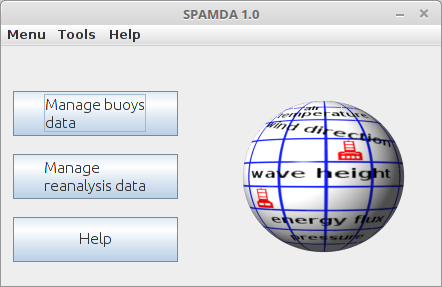
\includegraphics[scale=0.5]{figures/mainView.png}
			\caption{SPAMDA main view.}
			\label{fig:mainView}
		\end{figure}
			
		Such functional modules, which will be described in detail in the following sections, are accessible through the main view of SPAMDA represented in Fig. \ref{fig:mainView}.

		\section{Manage buoys data}

			The aim of this module is to provide the features for the management and analysis of the information related to the buoys from NDBC, since such information is entered in SPAMDA until it is used by the researchers for conducting their studies. Such management and analysis involves:
				\begin{itemize}
					\item Entering and updating the information of each buoy.
					\item The creation of the intermediate datasets with the collected measurements.
					\item Pre-processing tasks for obtaining the pre-processed datasets.
					\item The matching process to merge the information from NDBC and NNRP.
					\item The creation of the final datasets accordingly to the ML technique to use.
				\end{itemize}
				
			The following sections describe the organisation of this module.
			
			\subsection{Buoys}
			
				The \textit{Buoys} tab, which is represented in Fig. \ref{fig:tabBuoys}, allows the researchers to enter and update the information of each buoy. When entering a new buoy the following information, which can be obtained from NDBC, is requested:
				
				\begin{figure}[ht!]
					\centering
					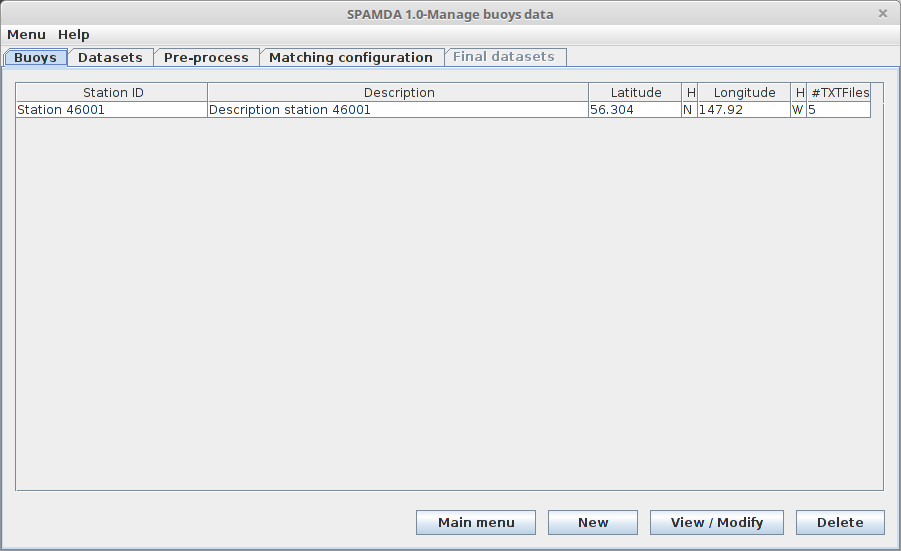
\includegraphics[scale=0.40]{figures/tabBuoys.png}
					\caption{Tab \textit{Buoys}.}
					\label{fig:tabBuoys}
				\end{figure}
				
				\begin{itemize}
					\item \textit{\textbf{Station ID}}: An alphanumeric identifier that allows the researchers to easily identify the buoy.
					\item \textit{\textbf{Description}}: A short description of the buoy.
					\item \textit{\textbf{Latitude}}: North or South geographical localisation (degrees) of the buoy. 
					\item \textit{\textbf{Longitude}}: West or East geographical localisation (degrees) of the buoy.
					\item \textit{\textbf{Measurements files}}: The above-mentioned annual text files of the standard meteorological information collected by the buoy and downloaded from NDBC web page, which will be used for the creation of the intermediate datasets. The researchers will add to the buoy one file per year and as many as needed. Remember that such files are available in NDBC web page \cite{NOAA_1}.
				\end{itemize}
				
				%To enter a new buoy click on \textcolor{blue}{\textit{New}} button, after typing the required information click on \textcolor{blue}{\textit{Save}} button for inserting the buoy. An example of entering a new boy is represented in Fig. \ref{fig:enteringBuoy}.
				
				To enter a new buoy follow the next steps:
				
					\begin{itemize}\itemsep0.02cm
						\item \textit{\textbf{Step 1}}: Click on the \textcolor{blue}{\textit{New}} button and the view represented in Fig. \ref{fig:enteringBuoy} will be displayed. (The remaining steps are related to such view).
						\item \textit{\textbf{Step 2}}: Type the required information about the buoy. To enter a new annual text file of the buoy click on the \textcolor{blue}{\textit{Add file}} button or click on the \textcolor{blue}{\textit{Delete file}} button to delete the selected one. By clicking on the \textcolor{blue}{\textit{Clear}} button it is possible to clean the form that request the information.
						\item \textit{\textbf{Step 3}}: Click on the \textcolor{blue}{\textit{Save}} button to insert the buoy.
					\end{itemize}
					
				%An example of entering a new boy is represented in Fig. \ref{fig:enteringBuoy}.
				
				\begin{figure}[ht!]
					\centering
					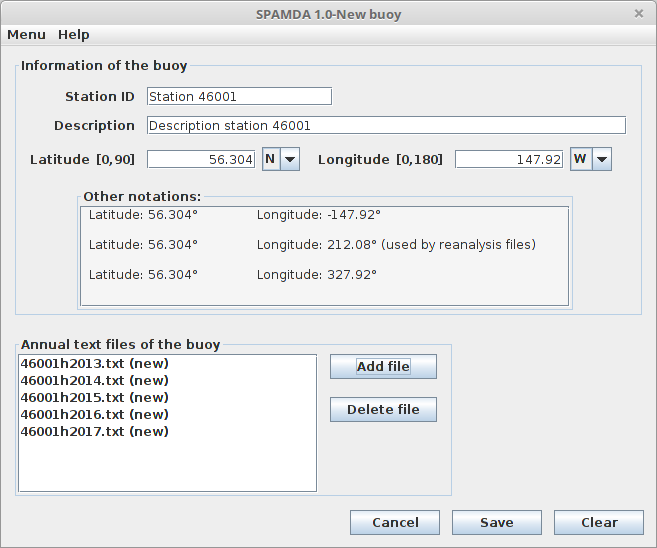
\includegraphics[scale=0.41]{figures/enteringBuoy.png}
					\caption{Entering a new buoy.}
					\label{fig:enteringBuoy}
				\end{figure}
				
				In the same way, by clicking on the \textcolor{blue}{\textit{View/Modify}} button it is possible to view or modify the data relating to the selected buoy. To delete a buoy click on the \textcolor{blue}{\textit{Delete}} button.
				
				\begin{center}
					\begin{warningbox}{Warning}{12cm}
						Deleting a buoy will remove all the data related to the buoy.
					\end{warningbox}
				\end{center}
				
			\subsection{Datasets}\label{sec:Datasets}
			
				%The \textit{Datasets} tab, which is represented in Fig. \ref{fig:tabDatasets}, allows the researchers to manage the intermediate datasets needed for their studies and relating to each buoy.
				
				The \textit{Datasets} tab, which is represented in Fig. \ref{fig:tabDatasets}, allows the researchers to manage the intermediate datasets of each buoy, which are the baseline for their studies.
				
				\begin{figure}[ht!]
					\centering
					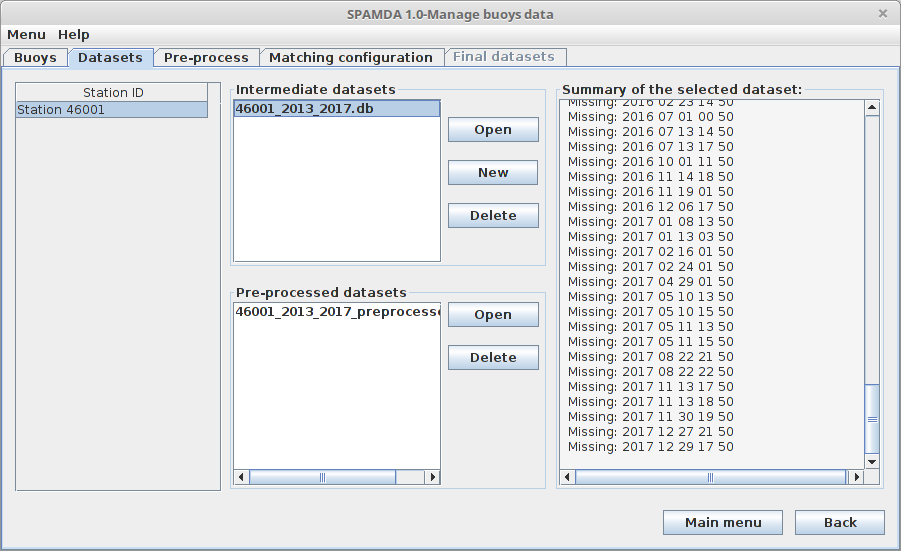
\includegraphics[scale=0.40]{figures/tabDatasets.png}
					\caption{Tab \textit{Datasets}.}
					\label{fig:tabDatasets}
				\end{figure}
			
				Once a buoy has been entered it is possible to create intermediate datasets using one ore more annual text files (added previously), which contain the measurements collected by the buoy. Note that such measurements may be incomplete or recorded at a different time than the expected one due to the weather conditions in which the buoys have to operate. SPAMDA has been designed to tackle such situation and it informs the researchers of any incidence found while reading the annual text files for creating the intermediate datasets.
				
				When an intermediate dataset is created, it is associated with its corresponding buoy, enabling the researchers to identify which intermediate datasets belong to each buoy. Besides, a summary of the content of the intermediate dataset is also created, providing relevant information about its content such as number of instances, date of first and last measurement, annual text files included, missing and duplicated dates.
				
				To proceed with the creation of an intermediate dataset follow the next steps:
				
					\begin{itemize}\itemsep0.02cm
						\item \textit{\textbf{Step 1}}: Select the desired buoy from the list shown on the left side.
						\item \textit{\textbf{Step 2}}: Click on the \textcolor{blue}{\textit{New}} button, then the view represented in Fig. \ref{fig:creatingIntermediateDataset} will be displayed. (The remaining steps are related to such view).
							\begin{figure}[ht!]
								\centering
								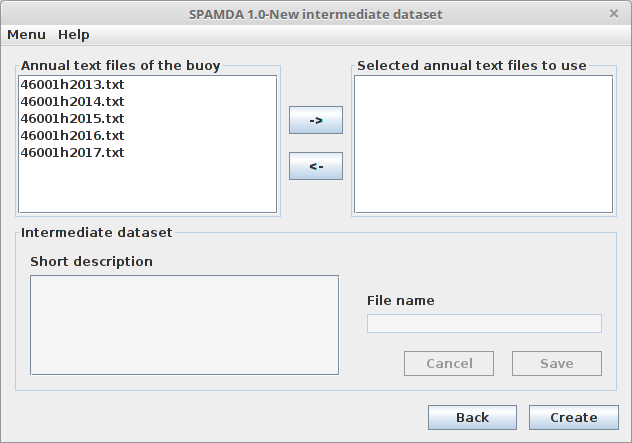
\includegraphics[scale=0.38]{figures/creatingIntermediateDataset.png}
								\caption{New intermediate dataset view.}
								\label{fig:creatingIntermediateDataset}
							\end{figure}
						\item \textit{\textbf{Step 3}}: Select the annual text files to use by clicking on the \textcolor{blue}{\textit{$-$$>$}} button. To deselect a previously selected file click on the \textcolor{blue}{\textit{$<$$-$}} button.
						\item \textit{\textbf{Step 4}}: When finished the selection click on the \textcolor{blue}{\textit{Create}} button.
						\item \textit{\textbf{Step 5}}: Type the description and the name of the intermediate dataset and click on the \textcolor{blue}{\textit{Save}} button to start the process of creation.
					\end{itemize}
					
				After that, SPAMDA will show the status of such process and the incidences that were found in the data, when it finished click on the \textcolor{blue}{\textit{Ok}} button. Note that the process can be cancelled by clicking on the \textcolor{blue}{\textit{Cancel creation}} button.
				
				The view that shows the status of the process of creation of an intermediate dataset for the buoy identified as \textit{Station 46001} using the annual text files of the years $2013$, $2014$, $2015$, $2016$ and $2017$ is represented in Fig. \ref{fig:statusCreationIntermediateDataset}.
			
					\begin{figure}[ht!]
						\centering
						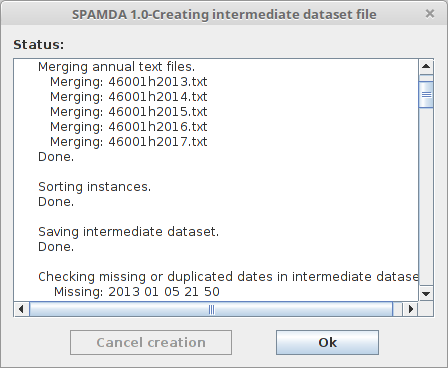
\includegraphics[scale=0.39]{figures/statusCreationIntermediateDataset.png}
						\caption{Status of the creation of the intermediate dataset.}
						\label{fig:statusCreationIntermediateDataset}
					\end{figure}
					
				%As it is shown in Fig. \ref{fig:tabDatasets} when a buoy is selected the intermediate datasets belonging to it are displayed, similarly occurs with the pre-processed datasets (which will be described in Section \ref{sec:Preprocess}) when selecting an intermediate dataset. Besides, on the right side is showed the summary of the intermediate or pre-processed dataset selected.
				
				As it is shown in Fig. \ref{fig:tabDatasets} when a buoy is selected, the intermediate datasets belonging to it are displayed, similarly, if one of these intermediate datasets  is selected, the pre-processed datasets (described in Section \ref{sec:Preprocess}) obtained from it are displayed. Besides, on the right side the summary of the intermediate or pre-processed dataset selected is shown.
				
				By clicking on the corresponding \textcolor{blue}{\textit{Delete}} button, the intermediate or pre-processed dataset selected will be removed.
				
				\begin{center}
					\begin{warningbox}{Warning}{13cm}
						Deleting an intermediate dataset will also remove all the pre-processed datasets belonging to it.
					\end{warningbox}
				\end{center}
				
				On the other hand, when clicking on the corresponding \textcolor{blue}{\textit{Open}} button the application will be redirected to the \textit{Pre-process} tab (see Section \ref{sec:Preprocess}) and the selected dataset (intermediate or pre-processed) will be opened for being pre-processed.
			
			\subsection{Pre-process}\label{sec:Preprocess}
			
				%The \textit{Preprocess} tab, which is represented in Fig. \ref{fig:tabPreprocess}, provides data pre-processing, which is useful for transforming raw data (intermediate datasets) into \textit{clean} and \textit{tidy} data. In this way, the quality of data can be improved prior to computational learning by ML techniques.
				
				The \textit{Pre-process} tab, which is represented in Fig. \ref{fig:tabPreprocess}, allows to perform data pre-processing, which prepares the raw data (intermediate datasets) to be able to be treated correctly by ML algorithms. In this way, the quality of data can be improved prior to computational learning.
				
				\begin{figure}[ht!]
					\centering
					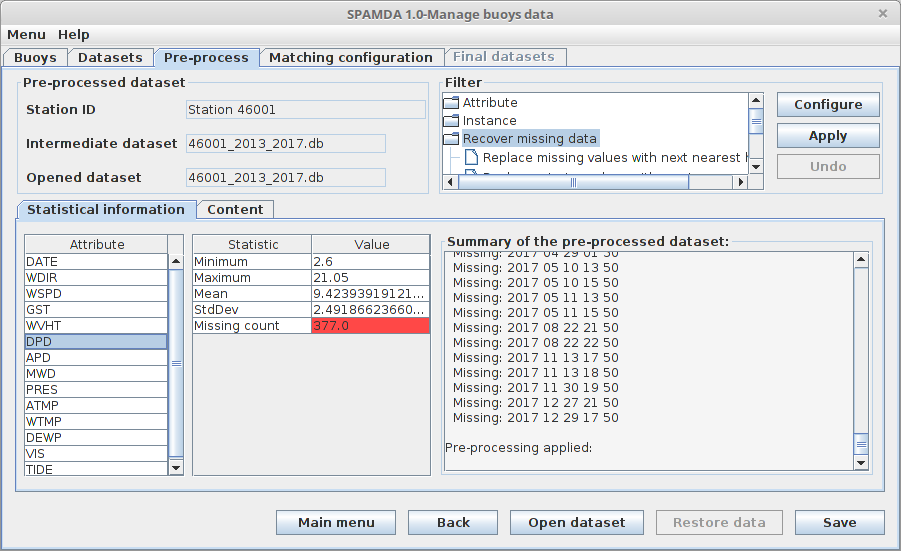
\includegraphics[scale=0.40]{figures/tabPreprocess.png}
					\caption{Tab \textit{Pre-process}.}
					\label{fig:tabPreprocess}
				\end{figure}
			
				Once an intermediate dataset has been created it is possible to apply the necessary pre-processing tasks (filters) to enhance the data quality. In the \textcolor{blue}{\textit{Statistical information}} tab relevant data about each attribute of the opened dataset (the one is currently being pre-processed) such as number of instances with missing values, minimum and maximum values, mean and standard deviation is shown. Providing the researchers the capacity to evaluate the pre-processing being performed.
				
				SPAMDA provides several configurable filters grouped in three categories, \textit{Attribute}, \textit{Instance} and \textit{Recover missing data}:
				
				\begin{itemize}
					\item \textit{Attribute}: All these filters can be applied to the attributes of the opened dataset.
						\begin{itemize}
							\item \textit{Normalize} \cite{WEKA_Filter_Normalize}: This filter normalises all numeric values of each attribute. The resulting values are by default in [0,1] for the data used to compute the normalisation intervals.
							\item \textit{Remove} \cite{WEKA_Filter_Remove}: It removes an attribute or a range of them.
							\item \textit{RemoveByName} \cite{WEKA_Filter_RemoveByName}: It allows to remove attributes based on a regular expression matched against their names.
							\item \textit{ReplaceMissingValues} \cite{WEKA_Filter_ReplaceMissingValues}: For each attribute all the missing values will be replaced with its mean.
							\item \textit{ReplaceMissingWithUserConstant} \cite{WEKA_Filter_ReplaceMissingWithUserConstant}: This filter replaces all the missing values of the attributes with an user-supplied constant value.
						\end{itemize}
				 \item \textit{Instance}: All these filters can be applied to the instances (hourly measurements) of the opened dataset.
					\begin{itemize}
						\item \textit{RemoveDuplicates} \cite{WEKA_Filter_RemoveDuplicates}: With this filter all duplicated instances are removed.
						\item \textit{RemoveWithValues} \cite{WEKA_Filter_RemoveWithValues}: This filter removes all the instances that match on the attribute and value user-supplied.
						\item \textit{SubsetByExpression} \cite{WEKA_Filter_SubsetByExpression}: It removes all the instances which don't match on a user-specified expression.
					\end{itemize}
				 \item \textit{Recover missing data}: All these filters can be applied to the instances of the opened dataset.
					\begin{itemize}
						\item \textit{Replace missing values with next nearest hour}: The missing values of each attribute are replaced with the next nearest non missing value.
						\item \textit{Replace missing values with previous nearest hour}: This filter replaces the missing values of each attribute with the previous nearest non missing value.
						\item \textit{Replace missing values with next $n$ hours mean}: The missing values of each attribute are replaced with the next $n$ nearest (configurable) non missing values mean. Note that these values may not coincide with the next $n$ hours.
						\item \textit{Replace missing values with previous $n$ hours mean}: This filter replaces the missing values of each attribute with the previous $n$ nearest non missing values mean. Note that these values may not coincide with the previous $n$ hours.
						\item \textit{Replace missing values with symmetric $n$ hours mean}: The missing values of each attribute are replaced with the $n$ previous and $n$ next non missing values mean. Note that these values may not coincide with the symmetric $n$ hours.
					\end{itemize}
				\end{itemize}
				
				%As a result of the data pre-processing it is possible to create new datasets, which are referenced as pre-processed datasets. Besides, a pre-processed dataset can be also pre-processed again enabling the researchers to resume such task at any other time.
				
				Once the pre-processing has been performed it is possible to save the resulting dataset, which will be referenced as a pre-processed dataset in SPAMDA. Besides, a pre-processed dataset can be also pre-processed again enabling the researchers to resume such task at any other time.
				
				To apply a filter follow the next steps:
				
					\begin{itemize}
						\item \textit{\textbf{Step 1}}: Open the desired intermediate or pre-processed dataset by clicking on either the \textcolor{blue}{\textit{Open dataset}} button or the corresponding \textcolor{blue}{\textit{Open}} button of tab \textit{Datasets}.
						\item \textit{\textbf{Step 2}}: Select one of the available filters.
						\item \textit{\textbf{Step 3}}: Configure the filter if necessary by clicking on the \textcolor{blue}{\textit{Configure}} button.
						\item \textit{\textbf{Step 4}}: Apply the filter by clicking on the \textcolor{blue}{\textit{Apply}} button.
					\end{itemize}
					
				As shown in Fig. \ref{fig:tabPreprocess} the pre-processing tasks performed on the opened dataset are displayed on the right side. SPAMDA allows the researchers to undo the last filter applied (\textcolor{blue}{\textit{Undo}} button) or to restore the initial content of the dataset (\textcolor{blue}{\textit{Restore data}} button).
				
				To create a pre-processed dataset follow the next steps:
				
					\begin{itemize}
						\item \textit{\textbf{Step 1}}: Click on the \textcolor{blue}{\textit{Save}} button, then the view represented in Fig. \ref{fig:creatingPreProcessedDataset} will be displayed. (The remaining step is related to such view).
							\begin{figure}[ht!]
								\centering
								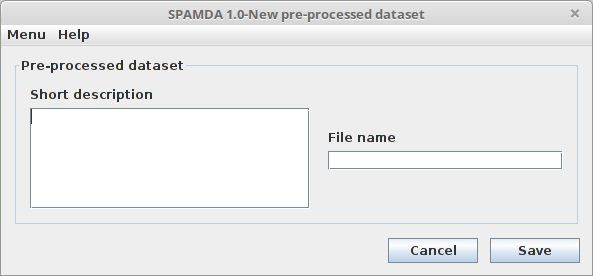
\includegraphics[scale=0.40]{figures/creatingPreProcessedDataset.png}
								\caption{New pre-processed dataset view.}
								\label{fig:creatingPreProcessedDataset}
							\end{figure}
						\item \textit{\textbf{Step 2}}: Type the description and the name of the pre-processed dataset and click on the \textcolor{blue}{\textit{Save}} button.
					\end{itemize}
					
				When saving the pre-processed dataset it will be associated with its corresponding intermediate dataset.

				Moreover, it is also possible to visualise the content of the opened dataset, enabling the researchers to easily identify if any of the instances is missing, duplicated, incomplete (missing values) or was recorded at a different time than the expected one, as mentioned in Section \ref{sec:Datasets}. To proceed with such action click on the \textcolor{blue}{\textit{Content}} tab and use the buttons \textcolor{blue}{\textit{$>$}} and \textcolor{blue}{\textit{$<$}} to check the possible affected instances as it is shown in Fig. \ref{fig:contentOpenedDataset}.
				
				\begin{figure}[ht!]
					\centering
					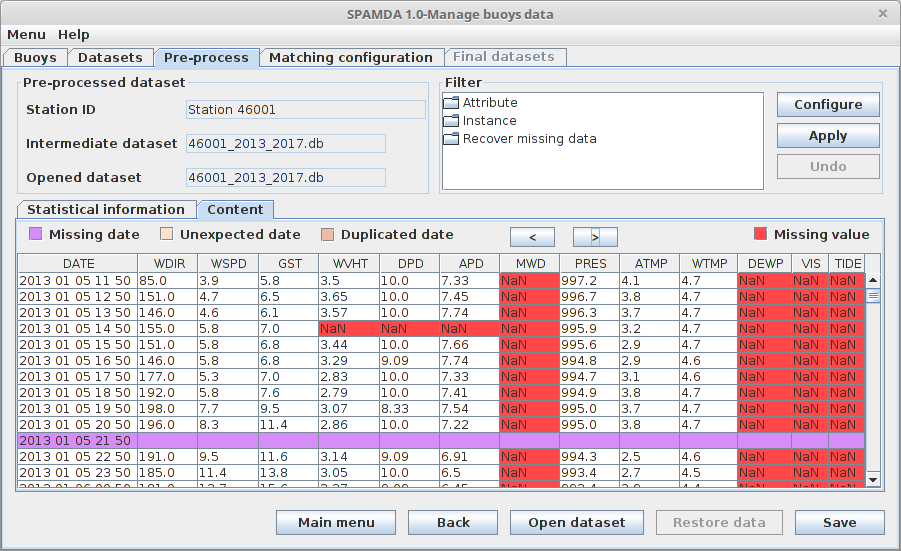
\includegraphics[scale=0.40]{figures/contentOpenedDataset.png}
					\caption{Visualising the content of the opened dataset.}
					\label{fig:contentOpenedDataset}
				\end{figure}
			
			\subsection{Matching configuration}\label{sec:MatchingConf}
			
				The \textit{Matching configuration} tab, which is represented in Fig. \ref{fig:tabMatchingConfiguration}, allows the researchers to customise the parameters of the matching process, which is necessary to carry out in order to merge and format the data provided by the two sources of information described in Section \ref{sec:DataSources}.
				
				\begin{figure}[ht!]
					\centering
					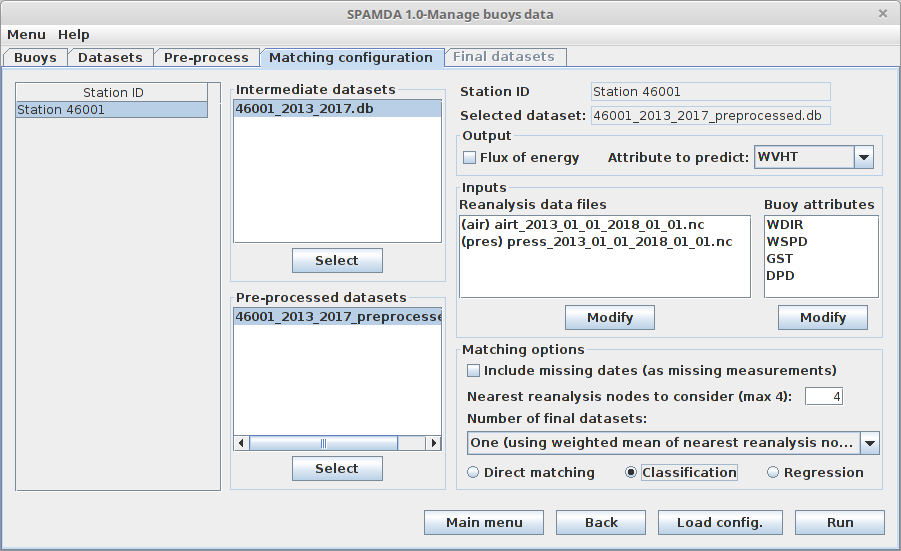
\includegraphics[scale=0.40]{figures/tabMatchingConfiguration.png}
					\caption{Tab \textit{Matching configuration}.}
					\label{fig:tabMatchingConfiguration}
				\end{figure}
			
				The matching procedure is performed using an intermediate or pre-processed dataset, which includes the measurements collected by a buoy from NDBC, and also the corresponding reanalysis data files from NNRP. Note that SPAMDA is able to manage the NetCDF binary format for handling the information stored in such reanalysis files.
				
				%Such process merges the information of both sources that matches on time, but due to that the measurements of the buoys are hourly collected from $00$:$50$ to $23$:$50$ UTC, and the reanalysis data is available every $6$ hours at $00$Z, $06$Z, $12$Z and $18$Z, the matching can only be carried out each $6$ hours (discarding the unused measurements from the buoy data). Besides, and since there is still a difference of 10 minutes, the matching with the reanalysis data will be performed with the nearest measurement (previous or next) within a maximum of 60 minutes of difference. Finally, the matched instances of both sources will result in the final datasets.
				
				Such process merges the information of both sources that match on time, but due to the measurements of the buoys are hourly collected from $00$:$50$ to $23$:$50$ UTC, and the reanalysis data is available every $6$ hours at $00$Z, $06$Z, $12$Z and $18$Z, the matching can only be carried out each $6$ hours (discarding the unused measurements from the buoy data). Besides, and since there is still a difference of 10 minutes, the matching with the reanalysis data will be performed with the nearest measurement (previous or next) within a maximum of 60 minutes of difference. Finally, the matched instances of both sources will result in the final datasets.
				
				SPAMDA allows the researchers to perform a customisable matching process, through which the researchers can easily obtain as different final datasets of the same meteorological data as needed, allowing them to consider different factors of the problem under study. These final datasets can be used for classification or regression prediction tasks, or direct matching. Prediction tasks are used to estimate the value of the output attribute in a concrete future using the information provided by the input attributes. Depending on the task to use, the final datasets must be prepared and configured in a specific way:
				
				\begin{itemize}
					\item \textit{Classification}: The final datasets will be ready to use as input in classification methods, which require a nominal output attribute and whose specific preparation is explained in Section \ref{sec:FinalDatasets}.
					\item \textit{Regression}: The final datasets will be ready to use as input in regression methods, which require a real output attribute and whose preparation is also explained in Section \ref{sec:FinalDatasets}.
					\item \textit{Direct matching}: In this case the inputs attributes have a direct correspondence with the output attribute, and it is not necessary to perform any additional preparation. For example, the final datasets may be used in lost data recovering tasks, or in the way the researchers consider suitable according to the problem under study.
				\end{itemize}
				
				Following, the parameters that can be configured in the matching process are described:
				
				\begin{itemize}
				
					\item \textit{Flux of energy} \cite{FERNANDEZ201544}: When the $F_e$ is selected, it will be used as output. This attribute is not collected by the buoys, but it can be calculated from two wave parameters: $H_s$ and $T_e$, which are collected as WVHT and APD attributes respectively. In this way, SPAMDA will obtain the $F_e$ of each instance using the following equation:
					
						\begin{equation}
							F_e = 0.49 \cdot H^2_s \cdot T_e
							\label{eq:fluxOfEnergy}
						\end{equation}
					
					where $F_e$ is measured in kilowatts per meter, $H_s$ is measured in meters and $T_e$ is measured in seconds. Note also that $F_e$ is defined in Eq. \ref{eq:fluxOfEnergy} as an average energy flux ($H_s$ is a kind of average wave height), though for simplicity it will be referred just as flux of energy.
					
					\item \textit{Attribute to predict}: Instead of using the $F_e$, the researchers can select any of the attributes collected by the buoys as output (e.g. significant wave height (WVHT), wind direction (WDIR), sea level pressure (PRES), etc.). Therefore, they can focus on different studies by selecting an attribute or other.

					\item \textit{Reanalysis data files}: In order to have a more accurate description of the problem under study, more than one reanalysis variable can be considered as input. Remember that these files have to be previously downloaded by the researcher from the website of the NNRP \cite{NNRP}, which should set the range of dates (temporal properties) and the desired sub-grid (spatial properties, see Fig. \ref{fig:subGrid}) for each variable of reanalysis. In that sense, the reanalysis data files must have the same spatial and temporal properties but relating to different variables each other.
					
					To select the needed reanalysis data files click on the corresponding \textcolor{blue}{\textit{Add/Modify}} button and the view represented in Fig. \ref{fig:selectingReanalysisDataFiles} will be displayed. SPAMDA facilitates this task by showing in cyan colour the reanalysis data files that are compatibles each other when selecting or clicking on a file. Click on the \textcolor{blue}{\textit{Confirm selection}} button when finished and SPAMDA will check that the selected files meet such condition.
					
					\begin{figure}[ht!]
						\centering
						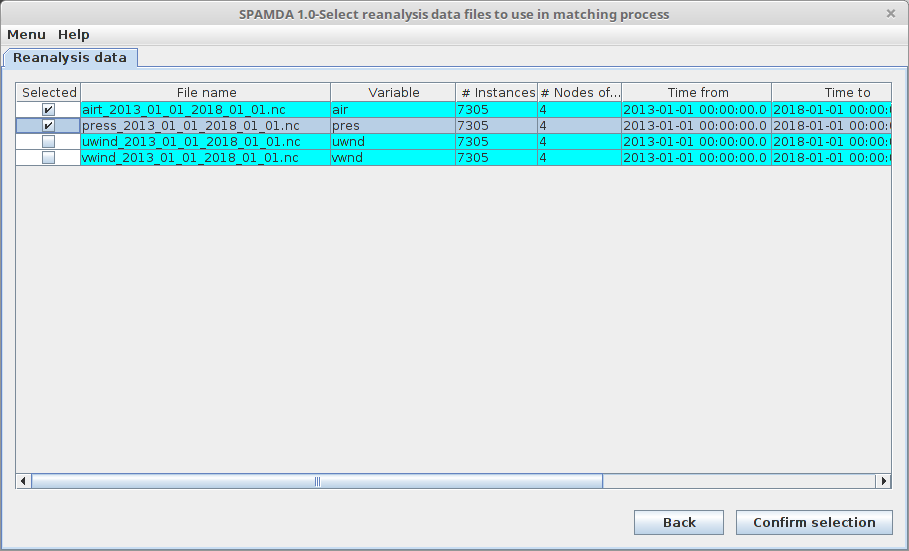
\includegraphics[scale=0.40]{figures/selectingReanalysisDataFiles.png}
						\caption{Selecting reanalysis data files.}
						\label{fig:selectingReanalysisDataFiles}
					\end{figure}

					\item \textit{Buoys attributes}: In addition to the reanalysis variables, the final datasets will also include the selected attributes as inputs (of the intermediate or pre-processed dataset used), providing a possible better characterisation of the problem under study, although it will depend on how correlated the attributes are.
					
					In the same way, in order to select the attributes of the buoy click on the corresponding \textcolor{blue}{\textit{Add/Modify}} button and the view represented in Fig. \ref{fig:selectingBuoysAttributes} will be displayed showing the available attributes of the buoy.
					
					\begin{figure}[ht!]
						\centering
						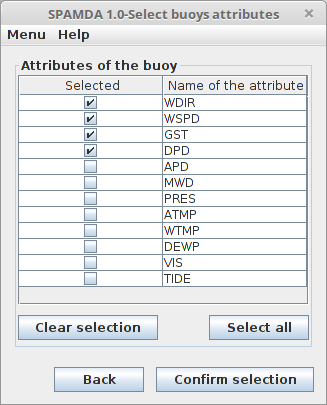
\includegraphics[scale=0.40]{figures/selectingBuoysAttributes.png}
						\caption{Selecting buoys attributes.}
						\label{fig:selectingBuoysAttributes}
					\end{figure}
					
					Once done the selection click on the \textcolor{blue}{\textit{Confirm selection}} button.
					
					\item \textit{Include missing dates}: As mentioned in Section \ref{sec:Datasets}, the information collected by a buoy may be incomplete due to measurements not recorded by it. As a consequence, the matching of instances between both sources of information may mismatch (missing dates). In that situation, the researchers can consider two options: 1) discard the instances affected or 2) include them. In the latter case, the final datasets will contain the affected instances, but the measurements of the buoy will be stored as missing values in WEKA format, denoted as \guillemotleft\textit{?}\guillemotright.
					
					\item \textit{Nearest reanalysis nodes to consider}: As already shown in Fig. \ref{fig:subGrid}, the reanalysis data files may contain information of several reanalysis nodes. In this way, this parameter allows the researchers to choose from:
					
						\begin{itemize}
						
							\item Consider all the reanalysis nodes: in this case, all the information of each selected reanalysis data file will be used.
							
							\item Consider only some of the reanalysis nodes: in this case, only the information of the $N$ closets reanalysis nodes (configurable) to the buoy will be used. To do that, SPAMDA uses the \textit{Haversine} formula \cite{Haversine_2009} to calculate the distance from each reanalysis node to the localisation of the buoy and obtain the closest ones. Haversine formula is also known as great circle distance, this formula perform calculation from main point to destination point with trigonometric function by using latitude and longitude. Haversine formula is calculated as follows:
							  \begin{linenomath*}
									\begin{equation}
										d(p_0,p_j)=\arccos(\sin(lat_0)\cdot \sin(lat_j)\cdot \cos(lon_0-lon_j) + \cos(lat_0) \cdot \cos(lat_j)),
										\label{eq:Haversine}
									\end{equation}
								\end{linenomath*}
							where $p_0$ is the buoy geographical localisation, $p_j$ stands for the location of each reanalysis node, and $lat$ and $lon$ are the latitude and longitude of the points, respectively.
							
						\end{itemize}
					
					\item \textit{Number of final datasets}: Depending on the number of the nearest reanalysis nodes to consider, the number of the final datasets to create and therefore the content of them can be configured according to the following options:

						\begin{itemize}
							%\item \textit{One (using weighted mean of $N$ nearest reanalysis nodes)}: Only one final dataset will be created, which will contain the attributes (the selected one as output and the selected ones as inputs) of the intermediate or pre-processed dataset used, along with a weighted mean of each variable of reanalysis used (one per selected reanalysis data file). This weighted mean takes into account the distance from each reanalysis node to the localisation of the buoy, and it is calculated by SPAMDA using the formula defined in Eq. \ref{eq:weightedMean}. Therefore, the closest reanalysis nodes to the localisation of the buoy will provide more information.
							
							\item \textit{One (using weighted mean of $N$ nearest reanalysis nodes)}: Only one final dataset will be created, which will contain the attributes (the selected one as output and the selected ones as inputs) of the intermediate or pre-processed dataset used, along with a weighted mean of each variable of reanalysis used (one per selected reanalysis data file). This weighted mean is obtained by SPAMDA and uses the distance (using the formula defined in Eq. \ref{eq:Haversine}) from each reanalysis node to the localisation of the buoy. Once the distances have been calculated they are inverted and normalised as follows:
							
								\begin{linenomath*}
									\begin{equation}
										w_i=\frac{\sum_{j=1}^{N} d(p_0,p_j)}{d(p_0,p_i)}, ~~i=1, \ldots, N.
										\label{eq:weightedMean}
									\end{equation}
								\end{linenomath*}
							
							After calculating these weights, they are applied to obtain a weighted mean of each variable of reanalysis. Therefore, the closest reanalysis nodes to the localisation of the buoy will provide more information.
							
							Considering as example the two nearest reanalysis nodes represented in Fig. \ref{fig:subGrid} and the reanalysis variables air temperature and pressure, the weighted mean of each reanalysis variable will be calculated using the reanalysis nodes $57.5$ N $\times$ $147.5$ W and $55.0$ N $\times$ $147.5$ W.
							
							\item \textit{'N' (one per each reanalysis node)}: As many final datasets as number of nearest $N$ reanalysis nodes configured by the researcher will be created. Therefore, each final dataset will contain the value of each reanalysis variable used of the nearest corresponding reanalysis node, along with the selected attributes of the intermediate or pre-processed dataset used.
							
							In this case, and considering as example the four closest reanalysis nodes (see Fig. \ref{fig:subGrid}) and the reanalysis variables air temperature and pressure, then only four final datasets will be created, containing each one the information of both reanalysis variables of the corresponding reanalysis node: $57.5$ N $\times$ $147.5$ W, $55.0$ N $\times$ $147.5$ W, $57.5$ N $\times$ $150.0$ W and $55.0$ N $\times$ $150.0$ W, along with the selected attributes of the intermediate or pre-processed dataset used.
							
						\end{itemize}
						
				\end{itemize}
				
				To proceed with the matching process follow the next steps:
				
					\begin{itemize}
						\item \textit{\textbf{Step 1}}: Select the desired buoy from the shown on the left side.
						\item \textit{\textbf{Step 2}}: Select the intermediate or pre-processed dataset to use.
						\item \textit{\textbf{Step 3}}: Configure the above-mentioned matching parameters and click on the \textcolor{blue}{\textit{Run}} button to start the matching process.
					\end{itemize}
					
				Then, SPAMDA will show the status of such process and the missing dates that were found, when it finished click on the \textcolor{blue}{\textit{OK}} button and the application will be redirected to the \textit{Final datasets} tab (see Section \ref{sec:FinalDatasets}) to perform the preparation of the matched data.
				
				In Fig. \ref{fig:statusMatchingProcess} is represented the status of a matching process using the configuration showed in Fig. \ref{fig:tabMatchingConfiguration}.
				
					\begin{figure}[ht!]
						\centering
						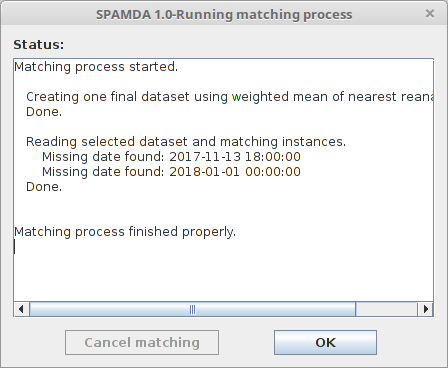
\includegraphics[scale=0.40]{figures/statusMatchingProcess.png}
						\caption{Status of the matching process.}
						\label{fig:statusMatchingProcess}
					\end{figure}
				
				Instead of typing all the required parameters, it is possible to load a previously matching configuration saved. To do that click on the \textcolor{blue}{\textit{Load config.}} button, then the view represented in Fig. \ref{fig:selectingMatchingConfiguration} will be displayed for selecting the configuration to be loaded (Section \ref{sec:FinalDatasets} describes how to save the configuration used in the matching process and for the preparation of the matched data).
				
				\begin{figure}[ht!]
					\centering
					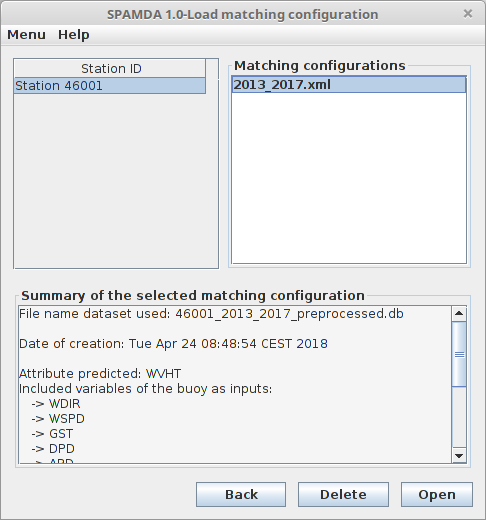
\includegraphics[scale=0.40]{figures/selectingMatchingConfiguration.png}
					\caption{Load matching configuration.}
					\label{fig:selectingMatchingConfiguration}
				\end{figure}
				

			\subsection{Final datasets}\label{sec:FinalDatasets}
			
				The \textit{Final datasets} tab, which is represented in Fig. \ref{fig:tabFinalDatasets}, permits the researchers to prepare the matched data for the desired prediction task (\textit{Regression} or \textit{Classification}), obtaining as a result the final datasets. Remember that \textit{Direct matching}, as it was described in Section \ref{sec:MatchingConf}, performs a direct correspondence between the attributes used as inputs and the output one, and it is not necessary to carry out any preparation.
				
				\begin{figure}[ht!]
					\centering
					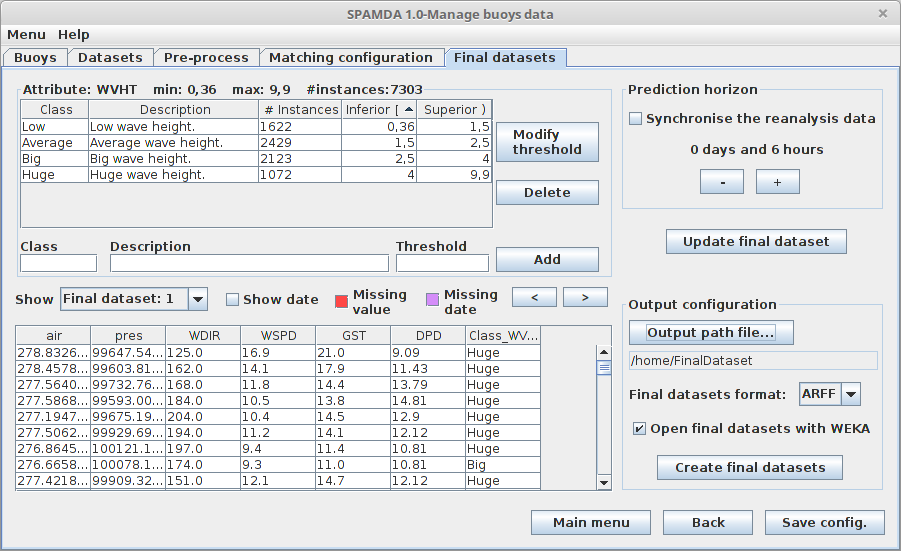
\includegraphics[scale=0.40]{figures/tabFinalDatasets.png}
					\caption{Tab \textit{Final datasets}.}
					\label{fig:tabFinalDatasets}
				\end{figure}
				
				SPAMDA allows the researchers to make such preparation by means of the following options:
				
					\begin{itemize}
						\item \textit{Prediction horizon} (Classification and Regression): This option indicates the time gap for moving backward the output attribute. In this way, the input attributes (variables of the buoy and reanalysis data) will be used to predict the output attribute in a concrete future (e.g. 6h, 12h, 18h, 1 day, etc.).
						
						The minimum interval for increasing and decreasing the prediction horizon is $6$h (due to reanalysis data temporal resolution) \cite{DORADOMORENO2017428}, the same interval used when the matching process is carried out. Therefore, for each increment of the prediction horizon an instance is lost from the end of the final datasets. As the minimum prediction horizon is $6$h at least one instance will be lost. The relation between the inputs and the attribute to predict will be defined as follows:
						
						\begin{linenomath*}
								\begin{equation}
									o_{t+\Delta t}=\phi(\mathbf{b}_t,\mathbf{r}_{t})
								\end{equation}
							\end{linenomath*}
						
						Where $t$ represents the time instant to study and $\Delta t$ the prediction horizon; $o$ is the attribute to predict, $\mathbf{b}$ is the vector containing the selected NDBC variables and $\mathbf{r}$ is the vector containing the selected reanalysis variables. Optionally, the reanalysis variables can be synchronised with the attribute to predict. Given that such variables are estimated by a mathematical model, it is allowed to use these future values, which could improve the performance of the results. In this case, the relation between the inputs and the attribute to predict would be:
						
							\begin{linenomath*}
								\begin{equation}
									o_{t+\Delta t}=\phi(\mathbf{b}_t,\mathbf{r}_{t+\Delta t})
								\end{equation}
							\end{linenomath*}
						
						\item \textit{Thresholds of the output attribute} (Classification): Since the values of the variables collected by the buoys are real numbers, it is necessary to discretise (convert from real to nominal values) the selected attribute as output. SPAMDA allows the researchers to perform this process by defining the necessary classes with their thresholds, which will be used against the values of the output attribute to carry out such discretisation.
					\end{itemize}
					
				Follow these steps to proceed with the preparation of the final datasets:
				
%					\begin{itemize}
%						\item \textit{\textbf{Step 1}}: Define the classes and its thresholds (\textit{Classification}).
%						\item \textit{\textbf{Step 2}}: Define the prediction horizon (\textit{Classification and Regression}).
%						\item \textit{\textbf{Step 3}}: Click on \textcolor{blue}{\textit{Update final dataset}} button.
%					\end{itemize}

					\begin{itemize}
						\item \textit{\textbf{Step 1}}: Define the classes and their thresholds (\textit{Classification}).
							\begin{itemize}
								\item To do that, use the buttons \textcolor{blue}{\textit{Add}}, \textcolor{blue}{\textit{Modify threshold}} or \textcolor{blue}{\textit{Delete}} to add a new threshold, modify or delete the selected one respectively.
							\end{itemize}
						\item \textit{\textbf{Step 2}}: Define the prediction horizon (\textit{Classification and Regression}).
							\begin{itemize}
								\item To do that, use the buttons \textcolor{blue}{\textit{$-$}} or \textcolor{blue}{\textit{$+$}} to decrease or increase the prediction horizon, and select or deselect the option \textcolor{blue}{\textit{Synchronise the reanalysis data}} depending on needs.
							\end{itemize}
						\item \textit{\textbf{Step 3}}: Click on the \textcolor{blue}{\textit{Update final dataset}} button to take the new configuration of the preparation.
					\end{itemize}
					
				Such preparation can be performed as many times as required and considering the typed options in each moment.
					
				As shown in Fig. \ref{fig:tabFinalDatasets}, the content of the final datasets obtained as a result of the custom preparation of the matched data, can be visualised enabling the researchers to check the final datasets before saving them on disk. Although the date will not be included in the final datasets, by selecting the \textcolor{blue}{\textit{Show date}} option it can be shown in order to know the dates of each instance of the intermediate or pre-processed dataset used, that matched with the reanalysis data. Moreover, by clicking on the \textcolor{blue}{\textit{$>$}} and \textcolor{blue}{\textit{$<$}} buttons it is possible to check the dates that were mismatched.

				Finally, and before creating the final datasets, it is necessary to define the output configuration:
			
				\begin{itemize}

					\item \textit{Output file}: Name of the final datasets and folder to save them on disk.
						
					\item \textit{Final datasets format}:

						\begin{itemize}
						
							\item \textit{ARFF}: \textit{Attribute-Relation File Format} \cite{WEKA_ARFF} which is used by the tool WEKA. SPAMDA allows the researchers to open the final datasets created with this format by running the environment Explorer of WEKA (in the same context of work), enabling they to choose the most appropriate ML method to tackle the problem under study. To do that select the option \textcolor{blue}{\textit{Open final datasets with WEKA}}.

							\item \textit{CSV}: \textit{Comma-Separated Values}. With this format the researchers may use the final datasets in the way they deem suitable.
							
						\end{itemize}
					
				\end{itemize}
				
				Once finished the preparation, by clicking on the \textcolor{blue}{\textit{Create final datasets}} button the final datasets will be saved on disk in the selected folder, an them will be opened by the tool WEKA, as represented in Fig. \ref{fig:openigFinalDatasetWeka}, if the researchers selected such option.
				
				\begin{figure}[ht!]
					\centering
					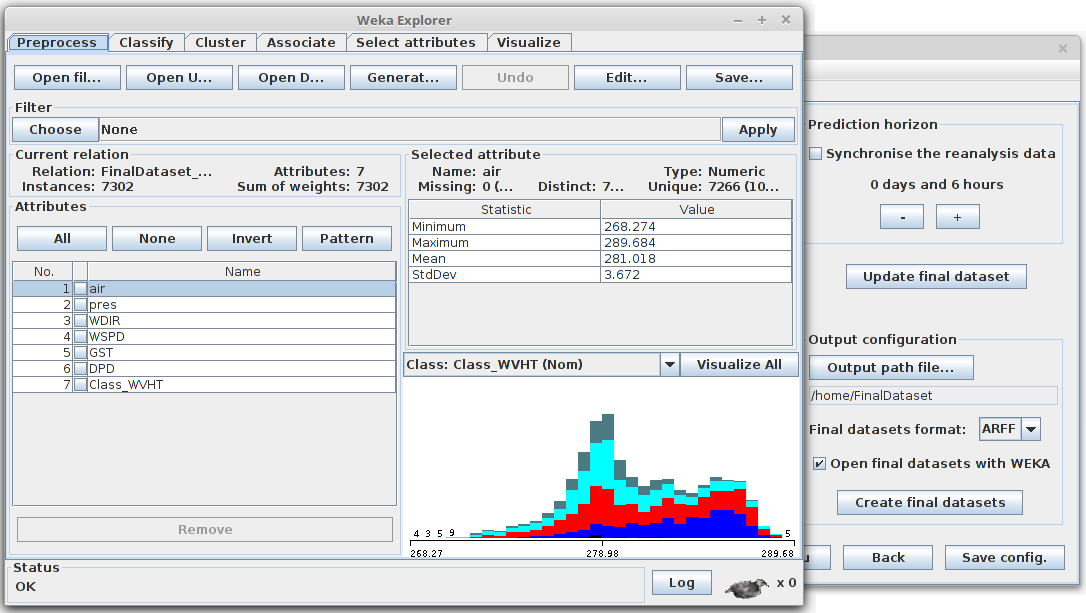
\includegraphics[scale=0.375]{figures/openigFinalDatasetWeka.png}
					\caption{Opening with WEKA the final dataset created.}
					\label{fig:openigFinalDatasetWeka}
				\end{figure}
				
				%Besides, a text file that summarises the configuration used in the matching process and for the preparation of the matched data is also generated in addition to the final datasets. 
				
				SPAMDA allows the researchers to save the configuration used in the matching process and for the preparation of the matched data, enabling the researchers to resume their studies at any other time. To do that click on the \textcolor{blue}{\textit{Save config.}} button, then the view represented in Fig. \ref{fig:creatingMatchingConfiguration} will be displayed. After typing the description and the file name click on the \textcolor{blue}{\textit{Save}} button to save the configuration, which will be associated with the buoy used.
				
				\begin{figure}[ht!]
					\centering
					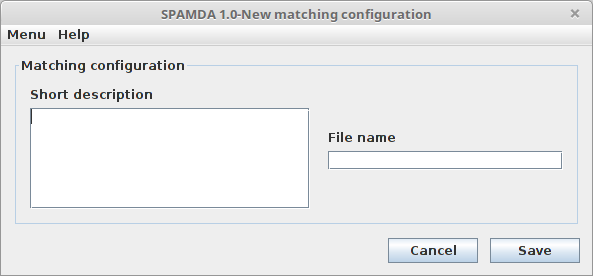
\includegraphics[scale=0.40]{figures/creatingMatchingConfiguration.png}
					\caption{New matching configuration.}
					\label{fig:creatingMatchingConfiguration}
				\end{figure}

		\section{Manage reanalysis data}
		
			This module, which is represented in Fig. \ref{fig:manageReanalysisData}, allows the management of the reanalysis data provided by NNRP. In this way, the researchers can keep up to date the reanalysis files needed for their studies. Remember that such data is available in NNRP web page \cite{NNRP}.
				\begin{figure}[ht!]
					\centering
					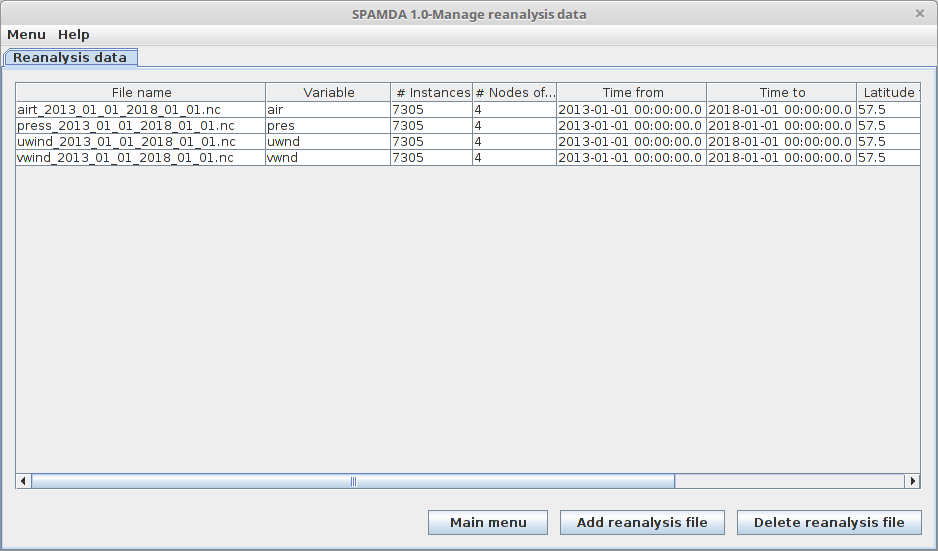
\includegraphics[scale=0.40]{figures/manageReanalysisData.png}
					\caption{Module Manage reanalysis data.}
					\label{fig:manageReanalysisData}
				\end{figure}
			
			To enter a new reanalysis file just click on the \textcolor{blue}{\textit{Add reanalysis file}} button and select the desired file, in order to delete a reanalysis file just click on the \textcolor{blue}{\textit{Delete reanalysis file}} button.
			
			As it is shown in Fig. \ref{fig:manageReanalysisData} useful information about the content of each reanalysis file can be consulted such as name of the file and the reanalysis variable, number of instances and reanalysis nodes, initial and final: time, latitude and longitude; which summarises the temporal and spatial properties of the data. Thus the researcher can quickly and easily identify each reanalysis file entered in SPAMDA.
		
		\section{Tools}
		
			This module includes two utilities, one for converting intermediate or pre-processed datasets to ARFF or CSV format and the other one for opening ARFF files with WEKA. Both features are accessible through the \textcolor{blue}{\textit{Tools}} option of the menu bar showed in Fig. \ref{fig:mainView}.
			
			\subsection{Datasets converter}
			
				This utility permits the researchers to convert the desired intermediate or pre-processed datasets to ARFF and CSV format. In this way, the researchers can use these converted datasets as they consider opportune.
				
				To convert an intermediate or pre-processed dataset click on the \textcolor{blue}{\textit{Dataset converter}} option and the view represented in Fig. \ref{fig:convertDatasets} will be displayed. On the left side are shown the buoys entered in SPAMDA, by clicking on one of them its intermediate datasets will be shown on the top side. Similarly, by clicking on one intermediate dataset its pre-processed datasets will be shown on the bottom side. Once selected the desired dataset (intermediate or pre-processed) just click on the \textcolor{blue}{\textit{Convert to ARFF}} or \textcolor{blue}{\textit{Convert to CSV}} button, and a dialog box will appear asking for the name of the target file that will be created as a result of the conversion.
				
					\begin{figure}[ht!]
						\centering
						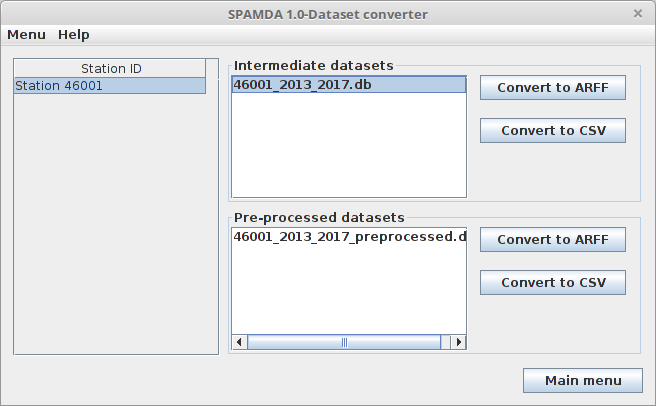
\includegraphics[scale=0.40]{figures/convertDatasets.png}
						\caption{Utility Dataset converter.}
						\label{fig:convertDatasets}
					\end{figure}
			
			\subsection{Open ARFF file with WEKA}
			
				This other utility allows the researchers to open ARFF files by running the environment Explorer of WEKA in the same context of work, enabling they to resume experiments with previously created final datasets.
				
				To open an ARFF file click on the \textcolor{blue}{\textit{Open ARFF file with WEKA}} option and the view represented in Fig. \ref{fig:openARFFfile} will be displayed.
				
					\begin{figure}[ht!]
						\centering
						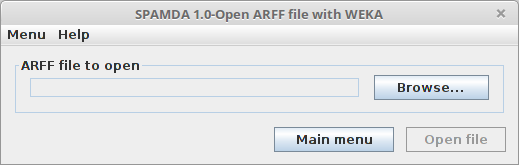
\includegraphics[scale=0.50]{figures/openARFFfile.png}
						\caption{Utility Open ARFF file with WEKA.}
						\label{fig:openARFFfile}
					\end{figure}
				
				To search for and select an ARFF file click on the \textcolor{blue}{\textit{Browse...}} button, when finished click on the \textcolor{blue}{\textit{Open file}} button for opening it and the view represented in Fig. \ref{fig:openingARFFFileWEKA} will be displayed.
					
					\begin{figure}[ht!]
						\centering
						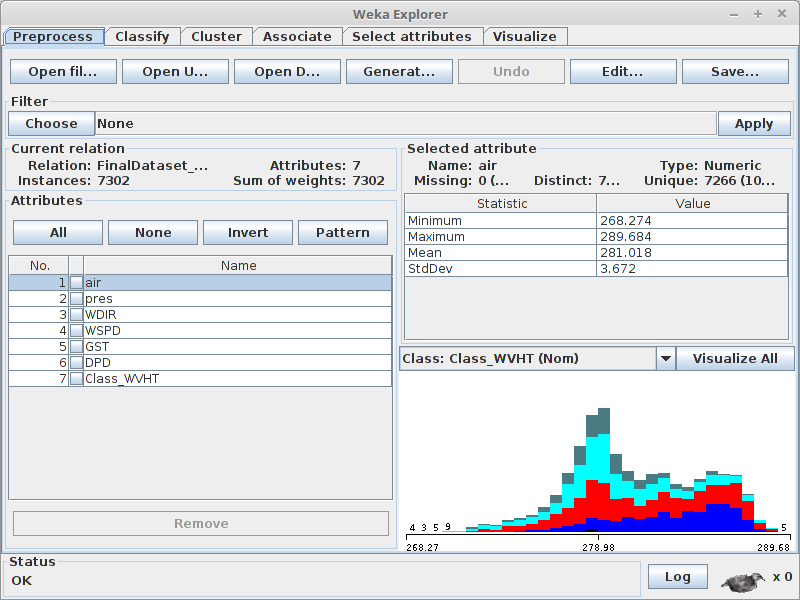
\includegraphics[scale=0.50]{figures/openingARFFFileWEKA.png}
						\caption{Opening an ARFF file with WEKA.}
						\label{fig:openingARFFFileWEKA}
					\end{figure}
					
				Remember that it is also possible to open the final datasets when creating them by selecting the option \textcolor{blue}{\textit{Open final datasets with WEKA}} (see Fig. \ref{fig:tabFinalDatasets}).
				
	\end{onehalfspace}
